%\begin{figure}[htp]
%	\centering
%	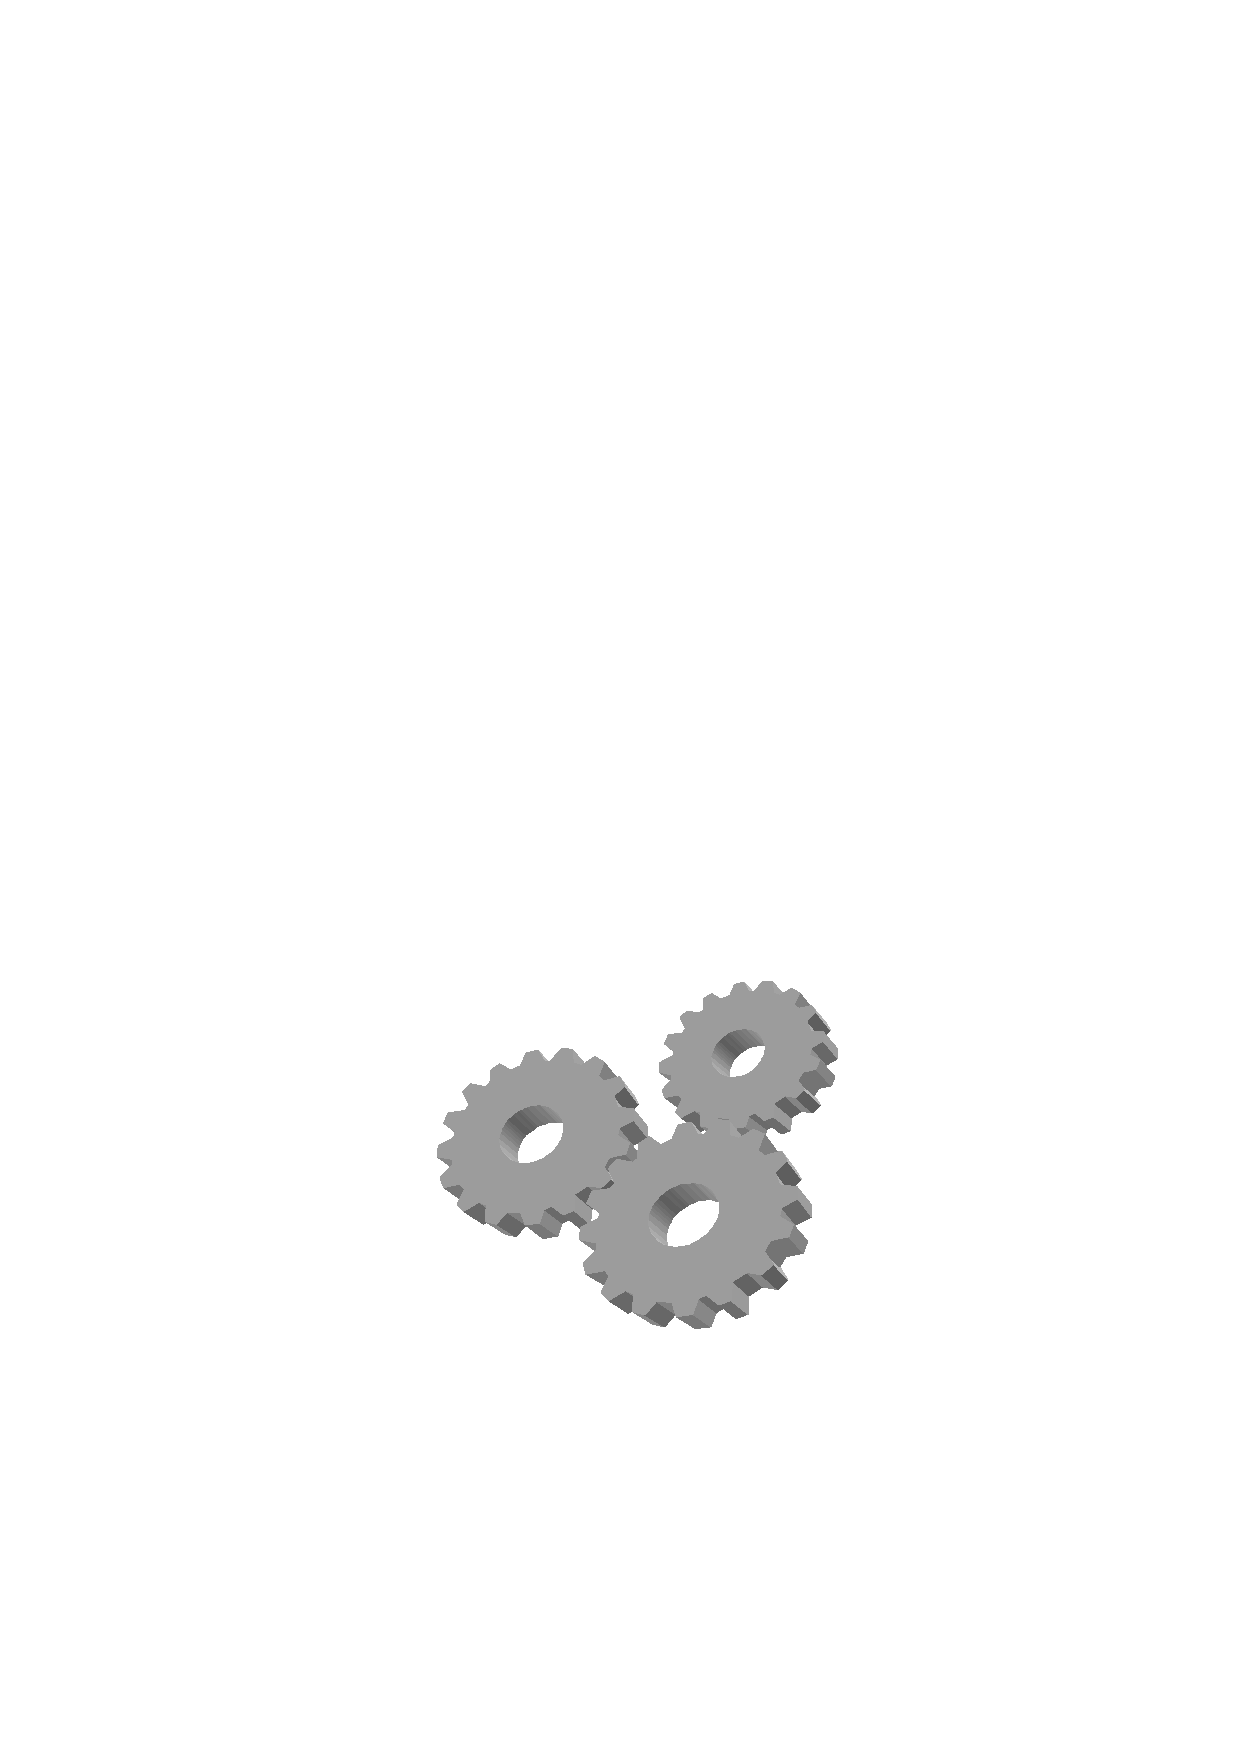
\includegraphics{picmain}
%	\caption{图 1.1 名称}
%\end{figure}

%\begin{table}[htp]
%	\centering
%	\begin{minipage}[t]{0.8\linewidth} % 如果想在表格中使用脚注,minipage是个不错的办法
%		\caption[表 1.1 名称]{}
%		\begin{tabular*}{\textwidth}{lp{10cm}}
%			\toprule[1.5pt]
%			{\hei 列1} & {\hei 列2} \\
%			\midrule[1pt]
%			&  \\
%			& \\
%			& \\
%			& \\
%			& \\
%			& \\
%			\bottomrule[1.5pt]
%		\end{tabular*}
%	\end{minipage}
%\end{table}

%\subsubsection{(1.1.1.1 题目)}


\chapter{非对称结构的实时跨模态RGB-D语义分割网络}



此处主要是与上一章节的逻辑联系。要写一页。

本章基于非对称的Transformer+Transformer结构,提出了一种轻量化的实时跨模态RGB-D语义分割网络CMFormer。具体而言,本章的主要工作包括几个部分:

(1)提出了一种基于非对称结构的跨模态RGB-D语义分割框架,分别处理RGB信息和深度信息的语义分割。
在RGB分支的VIT(Vision Transformer)中使用top-k稀疏注意力(top-k Sparse Attention, top-k SA),用以减少注意力机制计算时的信息冗余,降低模型大小,提高模型计算速度。
在RGB分支的VIT(Vision Transformer)使用轻量级的mix-transformer处理深度特征,该结构在处理深度信息的同时极大的压缩了模型大小。
	
(2)跨模态融合模块中使用特征选择模块,用以提取RGB模态和深度模态的有效信息。使用基于跨模态注意力引导的特征融合模块,用以融合RGB模态和深度模态,最后将融合的模态替换深度模态的原有信息。

(3)使用轻量级MLP解码器来解码浅层特征的语义信息,实现语义分割。



\section{模型方法}



\subsection{框架结构}
本章设计的CMFormer算法采用双分支结构处理RGB信息和深度信息,通过四个阶段的降采样对不同尺度的信息进行特征编码,采取中间层融合策略对不同尺寸的不同模态的信息进行融合,最后对融合的特征图进行解码实现RGB-D语义分割。

本章的算法主要有以下四个部分:基于top-k transformer的RGB信息处理分支、基于mix-transformer的深度信息处理分支、基于注意力引导的跨模态信息融合结构和轻量级的MLP解码器。如所示。
网络以三通道的RGB信息和三通道的深度信息作为输入,top-k transformer负责处理RGB信息,mix-transformer负责处理深度信息。由于第一阶段浅层特征比较明显,因此不进行特征融合,但是在之后的阶段都进行特征融合,基于注意力引导的跨模态信息融合结构负责融合不同阶段不同尺度的彩色信息和深度信息,将得到的融合信息放入深度信息处理通道。轻量级的MLP解码器负责第四阶段后的解码。


总体结构如\ref{图:efficient} 所示。
\begin{figure}[h]
	\centering
	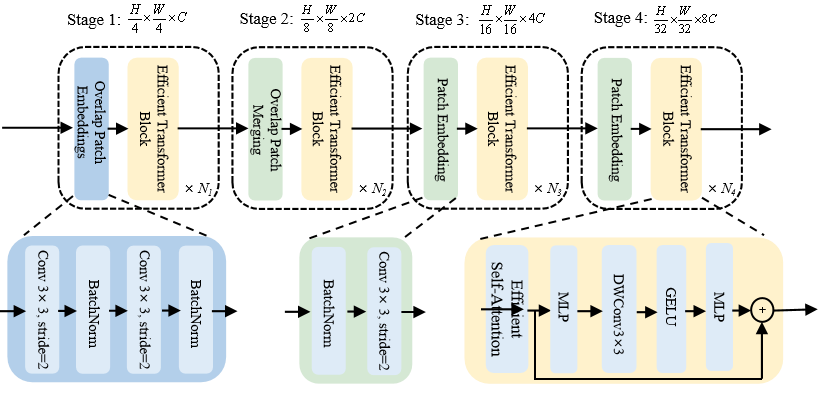
\includegraphics[width=\textwidth]{figures/efficient.png}
	\caption{efficient}
	\label{图:efficient}
\end{figure}


\subsection{基于top-k区域注意力机制的彩色信息处理分支}
常见的视觉transformer(vision transformer, VIT)在进行图像处理时,会先把图片切割成小块,然后将这些小块展平为序列作为输入。
VIT使用的是自注意力机制(Multi-Head Self-Attention, MHSA)。MHSA在进行计算的时候,需要计算输入序列中每个序列与其他所有序列之间的相似度,此时产生的计算复杂度为$O(N^2)$,其中, $N$是序列的长度,由小块的尺寸决定。
因此,在图片分辨率较大的时候,序列长度也较长,但是序列长度二次方增长的复杂度会导致计算量的急剧增长。
此外,在语义分割任务中,序列的分类更多的跟其周围的序列相关,不是所有的序列都有必要和其他的序列进行注意力的计算。

针对上述问题,本章算法提出基于top-k区域注意力机制(top-k regions attention,TRA)设计了处理彩色信息的视觉transformer。
top-k区域注意力原理如下:首先,将图片切割成包含若干个小块的区域。然后,计算区域之间的相似度,保留相似度最高的k个区域。最后,对区域内的小块使用稀疏注意力机制。top-k区域注意力机制的引入有效地减少了序列长度,降低了计算量。


划分区域。给定一个二维的特征图 $\mathbf{X} \in \mathbb{R}^{H \times W \times C}$,
将其划分为 $S \times S$个非不重合的区域,使每个区域包含 $\frac{HW}{S^2}$ 特征向量,
这时,$\mathbf{X}$重塑为$\mathbf{X}^r \in \mathbb{R}^{S^2 \times \frac{HW}{S^2} \times C}$,
继而通过线性投影可以得到$\mathbf{Q}, \mathbf{K}, \mathbf{V} \in \mathbb{R}^{S^2 \times \frac{HW}{S^2} \times C}$:
\begin{equation}
	\mathbf{Q} = \mathbf{X}^r \mathbf{W}^q, \; \;
	\mathbf{K} = \mathbf{X}^r \mathbf{W}^k, \; \;
	\mathbf{V} = \mathbf{X}^r \mathbf{W}^v,
\end{equation}
其中, $\mathbf{W}^q, \mathbf{W}^k, \mathbf{W}^v \in \mathbb{R}^{C \times C}$ 分别是$\mathbf{Q}, \mathbf{K}, \mathbf{V}$的投影权重。

选择top-k区域。通过构造有向图来选择与给定区域相关度排列最高的k个区域。
对之前得到的$\mathbf{Q}, \mathbf{K}$分别求取区域内的均值得到区域层面的$\mathbf{Q}^r, \mathbf{K}^r \in \mathbb{R}^{S^2 \times C}$,将$\mathbf{Q}^r$和$\mathbf{K}^r$的转置进行矩阵乘法运算可以得到邻接矩阵$\mathbf{A}^r \in \mathbb{R}^{S^2 \times S^2}$。
\begin{equation}
	\mathbf{A}^r = \mathbf{Q}^r (\mathbf{K}^r)^T. 
\end{equation}

邻接矩阵$\mathbf{A}^r$是两个区域语义相关的度量。
然后,通过为每个区域保留关联度最高的k个区域,得到稀疏邻接矩阵$\mathbf{I}_r \in \mathbb{N}^{S^2 \times k}$。
\begin{equation}
	\mathbf{I}^r = \mathrm{topkIndex}(\mathbf{A}^r).
\end{equation}
其中,$\mathbf{I}^r$ 的第$i$行包含了$k$个最相关区域的索引。

计算稀疏注意力。得到了稀疏邻接矩阵$\mathbf{I}_r$,就可以使用稀疏注意力。
首先,合并k个相关区域的$\mathbf{K}, \mathbf{V}$。
\begin{equation}
	\mathbf{K}^{g} = \mathrm{gather}(\mathbf{K}, \mathbf{I}^r), \; \; \mathbf{V}^g = \mathrm{gather}(\mathbf{V}, \mathbf{I}^r),
\end{equation}
其中,$\mathbf{K}^g, \mathbf{V}^g \in \mathbb{R}^{S^2 \times \frac{kHW}{S^2} \times C}$由k个相关区域对应参数合并产生。

然后,对收集的键值对使用稀疏注意力。
\begin{equation}
	\mathbf{O} = \mathrm{Attention}(\mathbf{Q}, \mathbf{K}^g, \mathbf{V}^g).
\end{equation}


复杂度的理论计算。
相比与普通注意力机制的复杂度$O((HW)^2)$,TRA的复杂度降低到了$O((HW)^\frac{4}{3})$。
TRA的复杂度计算包括三个部分:划分区域、选择top-k区域、计算稀疏注意力。
因此,总体的复杂度
\begin{equation}\label{eq:complexity}
	\begin{aligned}
		\mathrm{FLOPs} &= \mathrm{FLOPs}_{region} + \mathrm{FLOPs}_{top-k} + \mathrm{FLOPs}_{attention} \\
		&= 3HWC^2 + 2 (S^2)^2 C + 2HW k \frac{HW}{S^2} C \\
		&= 3HWC^2 + C (2S^4 + \frac{k(HW)^2}{S^2} + \frac{k(HW)^2}{S^2}) \\
		&\geq 3HWC^2 + 3C(2S^4 \cdot \frac{k(HW)^2}{S^2} \cdot \frac{k(HW)^2}{S^2})^\frac{1}{3} \\
		&= 3HWC^2 + 3Ck^\frac{2}{3}(2HW)^\frac{4}{3}
	\end{aligned}
\end{equation}

其中,$C$是特征映射的通道数,$k$是参与的区域数。公式中的放缩使用了均值不等式,当且仅当$2S^4 = \frac{k(HW)^2}{S^2}$时等式成立。
因此:
\begin{equation}\label{eq:condition}
	S = (\frac{k}{2}(HW)^2)^\frac{1}{6}.
\end{equation}

当根据公式\ref{eq:condition}划分区域大小时,TRA的复杂度可以降低到$O((HW)^\frac{4}{3})$。

TRA的伪代码如XX所示。
\begin{algorithm}[h]
	\caption{TRA}
	\label{alg:code}
	\begin{algorithmic}[1]
		\REQUIRE 特征图尺寸是(H, W, C)。
		$k$ 是区域数量。
		$S$ 区域数量的算术平方根。
		\ENSURE TRA处理后的特征图(H, W, C)。		
		\STATE $x = \mathit{patchify}(input, \mathit{patch\_size}=H//S)$
		\STATE $query, key, value = \mathit{linear\_qkv}(x).chunk(3, \mathit{dim}=-1)$
		\STATE $query\_r, key\_r = query.mean(\mathit{dim}=1), key.mean(\mathit{dim}=1)$
		\STATE $A_r = \mathit{mm}(query\_r, key\_r.transpose(-1, -2))$
		\STATE $I_r = \mathit{topk}(A_r, k).index$
		\STATE $key\_g = \mathit{gather}(key, I_r)$  
		\STATE $value\_g = \mathit{gather}(value, I_r)$  
		\STATE $A = \mathit{bmm}(query, key\_g.transpose(-2, -1))$
		\STATE $A = \mathit{softmax}(A, \mathit{dim}=-1)$
		\STATE $output = \mathit{bmm}(A, value\_g) + \mathit{dwconv}(value)$
		\STATE $output = \mathit{unpatchify}(output, \mathit{patch\_size}=H//S)$
	\end{algorithmic}
\end{algorithm}

TRA过程如图如\ref{图:top-k区域注意力机制} 所示。
\begin{figure}[h]
	\centering
	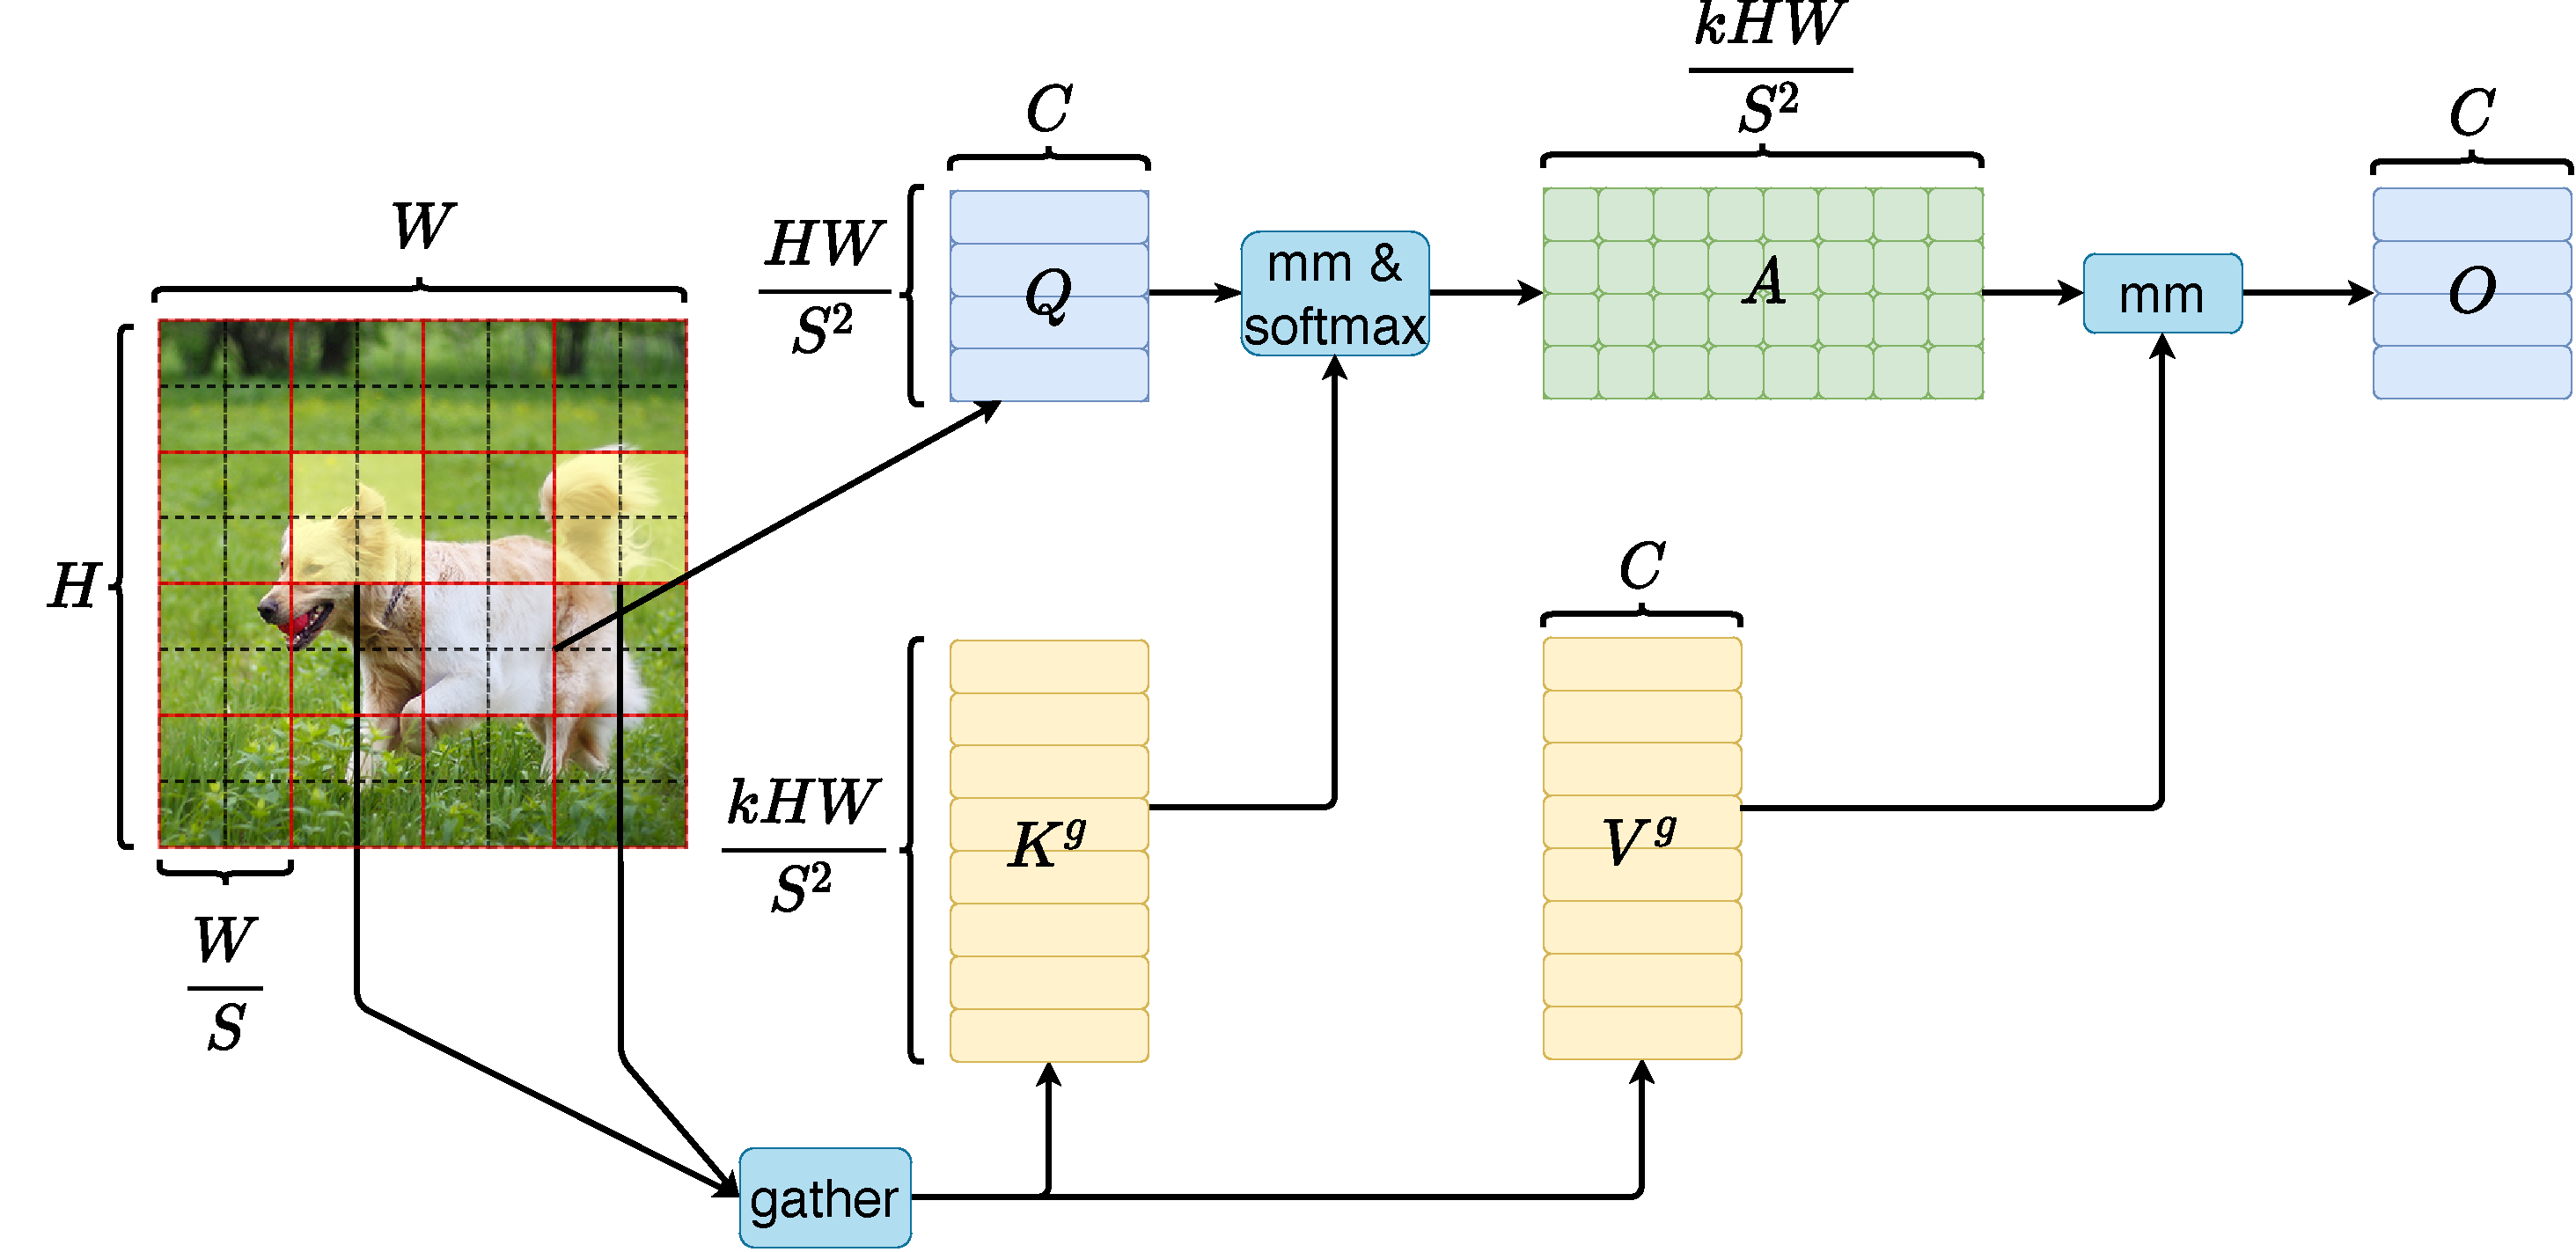
\includegraphics[width=\textwidth]{figures/top-k区域注意力机制.pdf}
	\caption{top-k区域注意力机制}
	\label{图:top-k区域注意力机制}
\end{figure}

基于TRA的视觉transofrmer如图如\ref{图:基于top-k区域注意力机制的RGB处理分支}所示。
\begin{figure}[h]
	\centering
	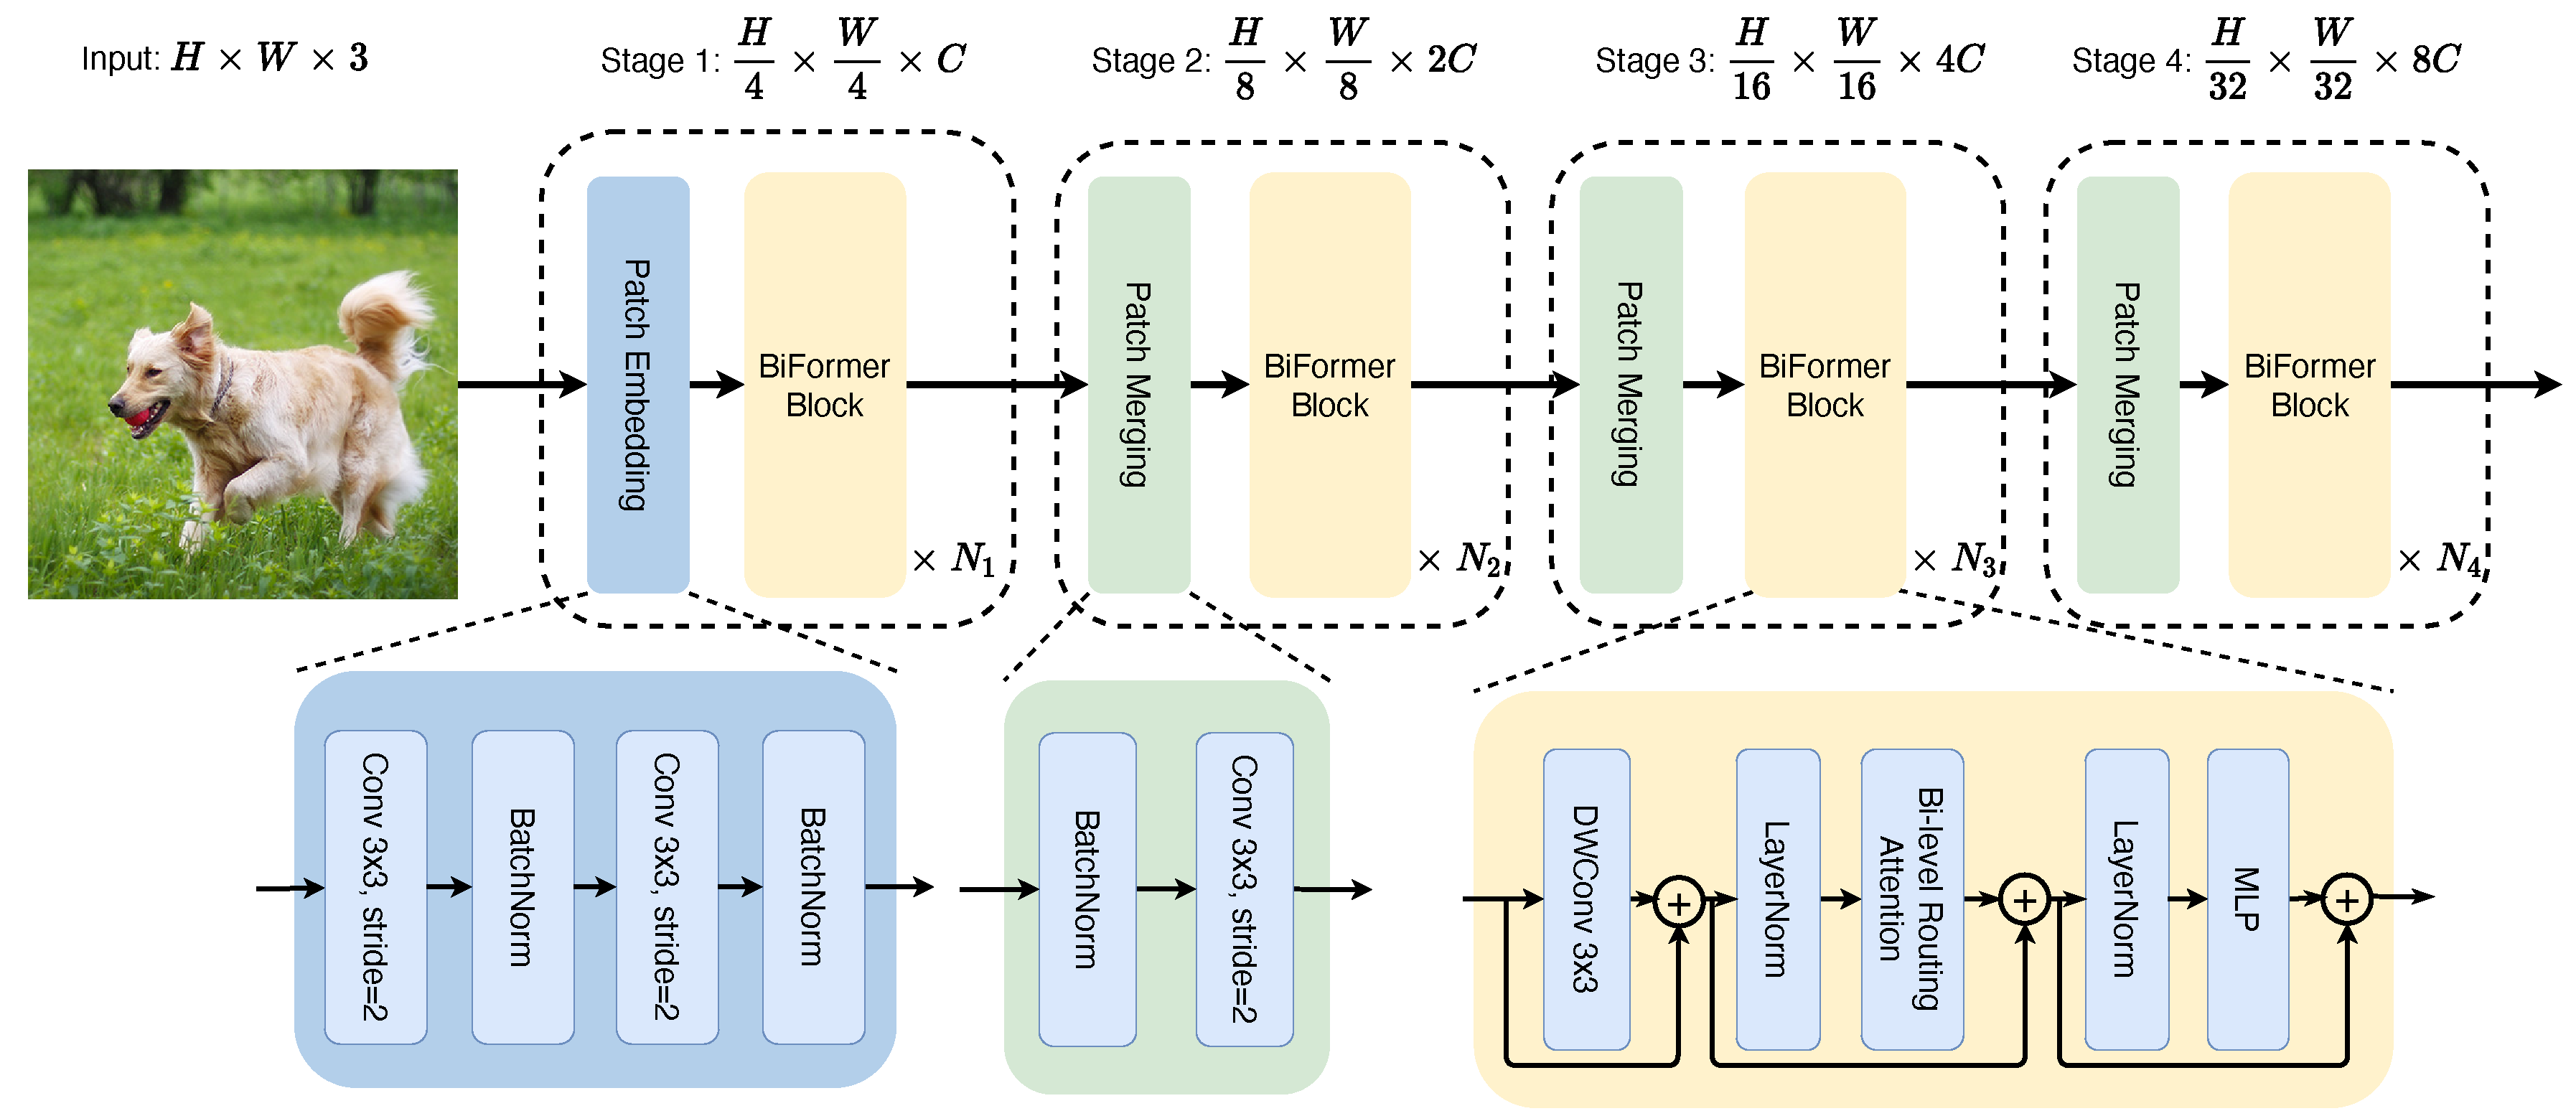
\includegraphics[width=\textwidth]{figures/基于top-k区域注意力机制的RGB处理分支.pdf}
	\caption{基于top-k区域注意力机制的RGB处理分支}
	\label{图:基于top-k区域注意力机制的RGB处理分支}
\end{figure}




\subsection{基于稀疏自注意力的深度信息处理分支}
VIT依靠多头自注意力机制强大的特征提取能力,对输入信息进行高效特征提取,在语义分割领域取得了很好的进展。
但是,不同于三通道的彩色信息,深度信息是单通道的,所以其包含的有效信息比彩色信息更少。

针对这个问题,本文在深度信息处理分支,改进VIT使用的自注意力机制,
使用稀疏自注意力构建更高效的transformer,获取更加轻量化的语义分割模型。


%\textbf{(1)稀疏自注意力。}
%
%在本章,对自注意力机制进行改进,使用稀疏自注意力机制,组成轻量级的transformer块嵌入到编码器中,用较低的计算成本来完成语义分割任务。

\textbf{(1)重叠补丁嵌入。}
对于一个输入的图片来说,ViT使用的不重叠的补丁嵌入操作,将一个$N \times N \times 3$的补丁统一为一个$1 \times 1 \times C$的向量。
这种操作可以很容易地将一个$2 \times 2 \times C_i$的特征统一为$1 \times 1 \times C_{i+1}$的向量,从而获得分层特征映射。
因此,我们可以将不同的层次特征不断缩小,从而获得预期大小尺寸的特征映射。
但是,不重叠的补丁嵌入不能保证补丁的局部连续性。
因此,我们使用重叠补丁嵌入。
通过定义补丁大小、两个相邻补丁之间的步幅和填充大小,可以产生与不重叠补丁嵌入一样大小的特征。
重叠补丁嵌入如\ref{图:补丁嵌入} 所示。
\begin{figure}[h]
	\centering%
	\subfloat[非重叠补丁嵌入]{%
		\label{fig:rescue_1}
		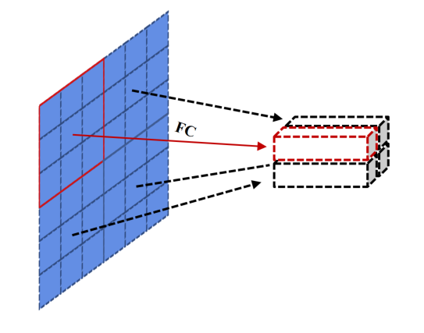
\includegraphics[width=0.5\textwidth]{figures/非重叠补丁嵌入.png}}
	\subfloat[重叠补丁嵌入]{%
		\label{fig:rescue_3}
		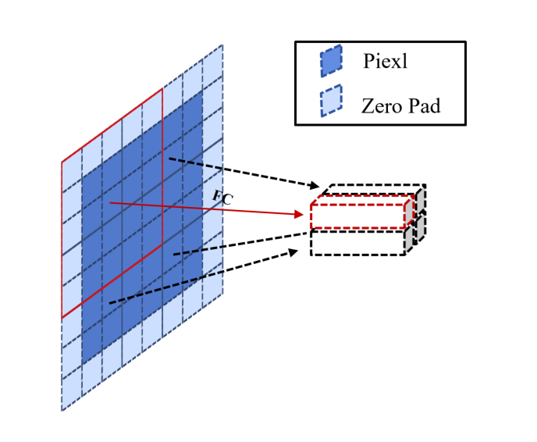
\includegraphics[width=0.5\textwidth]{figures/重叠补丁嵌入.png}}
	\vspace{-1em}
	\caption{补丁嵌入}
	\label{图:补丁嵌入}
\end{figure}



\textbf{(2)稀疏自注意力。}
传统的自注意力机制如下所示:
\begin{equation}
	{\rm Attention}({Q}, {K}, {V}) = {\rm Softmax}(\frac{{Q}{K}^\mathsf{T}}{\sqrt{d_{head}}}){V}.
	\label{eqn:mhsa}
\end{equation}

本文采用XX介绍的序列简约算法,该算法使用稀疏因子R来缩减序列的长度。如下所示:
\begin{equation}
	\begin{aligned}
		&{\hat{K}} = {\text{Reshape}(\frac{N}{R},C \cdot R)(K)}\\
		&{K} = {\text{Linear}(C \cdot R, C)({\hat{K}}),}
	\end{aligned}
	\label{eqn:reduce}
\end{equation}

其中,$K$是待稀疏的序列,$R$是一个固定的稀疏因子。在实验中的阶段1到阶段4,$R$被设定为[64,~16,~4,~1]。
在上述公式中,第一个公式将$K$的形状由$N \times C$重塑为$\frac{N}{R}\times (C \cdot R)$,
第二个公式将重塑的$K$线性操作,将其形状展开为$\frac{N}{R} \times C$。
因此,该操作可以使自注意机制的复杂性从$O(N^2)$降低到$O(\frac{N^2}{R})$。
如\ref{图:稀疏自注意力} 所示。
\begin{figure}[h]
	\centering
	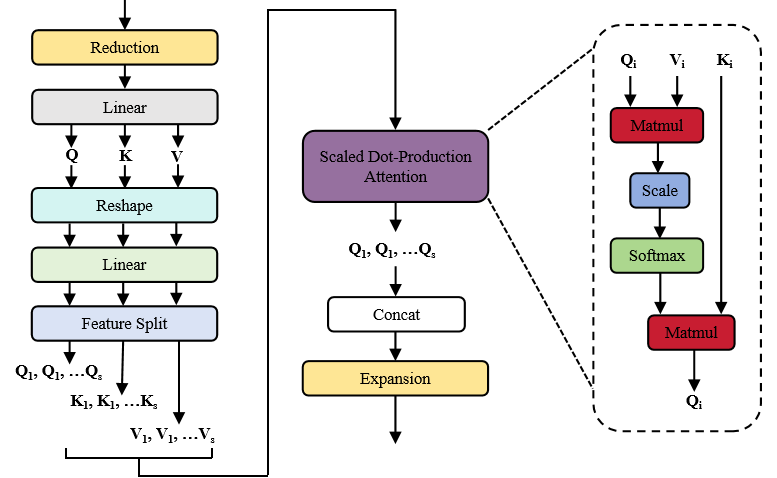
\includegraphics[width=\textwidth]{figures/稀疏自注意力.png}
	\caption{稀疏自注意力}
	\label{图:稀疏自注意力}
\end{figure}






\textbf{(3)高效的前馈网络。}
在VIT中使用的传统Transformer模型中,
由于注意力机制并没有考虑图片小块的先后顺序信息,
因此需要通过位置编码(Positional Encoding,PE)这种方式把前后的位置信息加在输入的图片小块上,
这样让Transformer保留图片小块的位置信息,可以提高模型对序列的理解能力。
然而,位置编码的分辨率是固定的。
因此,当测试分辨率与训练分辨率不同时,需要对位置编码进行插值,这往往会导致预测准确性下降。


为了缓解这个问题,
本文引入Mix-FFN(Mixed Feed-Forward Network),
该结构考虑了零填充对泄漏位置信息的影响,通过在前馈网络中直接使用3 × 3卷积来实现位置编码。

传统的FFN在每个位置上都采用相同的非线性变换,而Mix-FFN则允许对不同位置应用不同的非线性变换,从而增强模型的表达能力。
具体来说,Mix-FFN使用了全局前馈神经网络(Global FFN)和局部前馈神经网络(Local FFN)两种不同的前馈神经网络结构。
全局FFN是一个具有较大感受野的前馈神经网络,能够更好地捕捉全局上下文信息。
而局部FFN是一个具有较小感受野的前馈神经网络,能够更好地捕捉局部细节信息。 通过同时使用全局FFN和局部FFN,Mix-FFN能够在处理不同位置的特征时更加灵活和准确。
全局FFN可以帮助模型捕捉到更长范围的依赖关系和语义信息,而局部FFN则可以更好地处理局部细节和细微变化。
此外,Mix-FFN在每个FFN中将一个3 × 3卷积和一个MLP混合在一起,该结构可以为Transformer提供位置信息。
并且,我们使用深度可分离卷积来减少参数数量并提高效率。
Mix-FFN可以表示为:
\begin{equation}
	{\mathbf{x}_{out} = {\text{MLP(GELU}(\text{Conv}_{\text{3} \times \text{3}}(\text{MLP}(\mathbf{x}_{in}))))+ \mathbf{x}_{in}},}
	\label{eqn:mixffn}
\end{equation}

Mix-FFN如\ref{图:mixffn} 所示。
\begin{figure}[h]
	\centering
	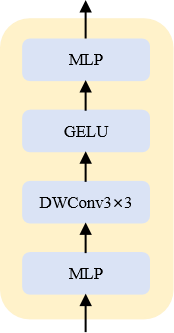
\includegraphics[width=0.25\textwidth]{figures/mixffn.png}
	\caption{mixffn}
	\label{图:mixffn}
\end{figure}


\textbf{(4)网络结构}
网络结构如\ref{图:efficient} 所示。
\begin{figure}[h]
	\centering
	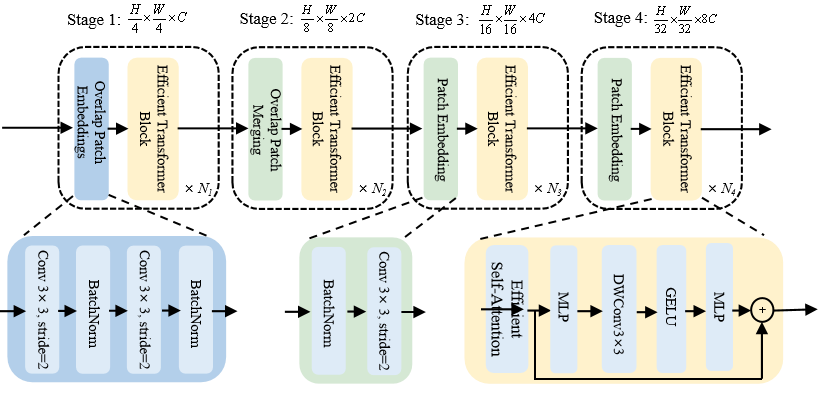
\includegraphics[width=\textwidth]{figures/efficient.png}
	\caption{efficient}
	\label{图:efficient}
\end{figure}





\subsection{基于交叉注意力的跨模态特征融合}
\textbf{(1)基于空间和通道注意力的跨模态特征选择}

空间注意力和通道注意力可以从特定模态中压缩特征并选择特征,提高语义分割的准确性。但是,现有的空间注意力和通道注意力机制采取不可学习的方法来压缩特征,这种方法对单模态的特征选择较为充分,但是对多模态输入,就无法兼顾不同模态特征之间的差异性,进而不利于不同模态信息的利用。

针对上述问题,本文提出基于空间和通道注意力的跨模态特征选择方法。该方法通过可学习的策略对彩色信息和深度信息进行特征压缩和特征选择。

首先,对彩色信息和深度信息拼接的特征图进行均值池化和最大池化,并将两种池化信息加权求和得到特征图的全局信息向量。其次,在通道注意力部分,全局信息向量被输入到一个多层感知机用来产生表示不同通道的权重分配向量,然后将权重分配向量通过Sigmoid函数得到归一化的通道注意力权重。在空间注意力部分,全局信息向量被输入到另一个多层感知机产生表示不同通道的权重分配向量,通过与原始特征图相乘后在通道维度的相加,可以得到不同空间的空间权重分配向量,然后将空间权重分配向量通过Sigmoid函数得到归一化的空间注意力权重。最后,将原始特征图和通道注意力权重和空间注意力权重相乘得到跨模态的融合特征。

如图如\ref{图:特征选择}所示。
\begin{figure}[h]
	\centering
	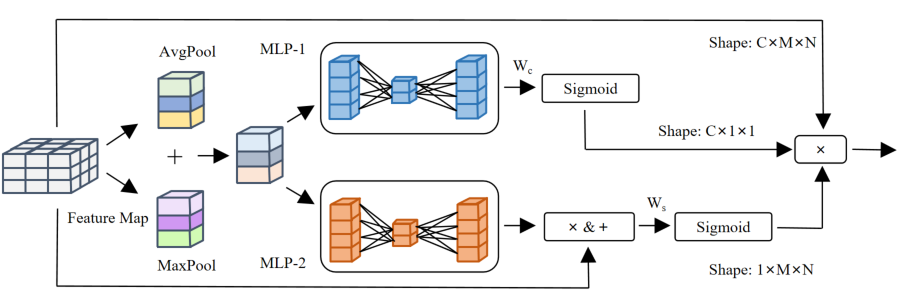
\includegraphics[width=\textwidth]{figures/特征选择.png}
	\caption{基于空间和通道注意力引导的跨模态特征选择}
	\label{图:特征选择}
\end{figure}


\textbf{(2)基于交叉注意力的跨模态特征嵌入}

VIT利用transformer中的多头注意力(MultiHead Self-Attention, MHSA)对输入的模态信息进行特征提取。
但是MHSA只接受单一模态的信息,因而只能对同一模态的信息进行自相似性计算。
在跨模态的语义分割任务中,单一模态的自相似性计算无法对来自不同模态的信息进行特征提取,因此无法充分利用来自不同模态信息的互补性来提高语义分割的性能。


针对这一问题,本文提出基于交叉注意力的跨模态特征嵌入方法。
该方法借鉴自注意力机制中的自相似性计算,通过定义跨模态自相似性构造交叉注意力机制,提出一个跨模态特征嵌入模块,从而对彩色信息和深度信息进行特征融合。

\textbf{特征混合重组。}
跨模态特征嵌入模块有三个输入,分别是彩色特征,深度特征和融合特征。
首先,彩色特征和深度特征会被投影到向量子空间中,用来产生对应模态的$Key$和$Query$。
融合特征会被投影到第三个向量子空间中,用来产生融合模态对应的$Value$。
如XX所示。


然后,如果在不同的子空间中计算自相似性,那么就无法在不同的子空间同时包含彩色信息和深度信息包含的特征。
因此,为了可以从不同的特征子空间学习特征,利用混合重组方法将彩色信息和深度信息产生的$Key$拼接后打乱重组。
这样,新产生的$Key$就同时包含了来自彩色模态和深度模态的信息。将彩色信息和深度信息产生的$Query$拼接后打乱重组。这样,新产生的$Query$也同时包含了来自彩色模态和深度模态的信息。
如XX所示。

\textbf{跨模态自相似性。}
假设彩色信息和深度信息的特征被编码为 $Key$ 和 $Query$,那么对于任意一个像素 $(i_0,j_0)$,它与其他像素 $(i,j)$ 的跨模态自相似性可以被定义为:
\begin{equation}
	W(i,j)=\sum_{n=1}^{N}(Krgb_{n,i,j} \cdot Qrgb_{n,i_0,j_0})+\sum_{n=1}^{N}(Kdepth_{n,i,j} \cdot Qdepth_{n,i_0,j_0})\
\end{equation}

其中, 
$Krgb_{n,i,j}$表示像素$(i_0,j_0)$产生的$Key$在彩色模态的第$n$个特征值,
$Qrgb_{n,i,j}$表示像素$(i_0,j_0)$产生的$Query$在彩色模态的第$n$个特征值,
$Kdepth_{n,i,j}$表示像素$(i_0,j_0)$产生的$Key$在深度模态的第$n$个特征值,
$Qdepth_{n,i,j}$表示像素$(i_0,j_0)$产生的$Query$在深度模态的第$n$个特征值。

\textbf{跨模态交叉注意力。}
在计算完跨模态自相似性后,还需要将计算的结果嵌入到融合特征$Value$中。
首先,计算$K_1$和$Q_1$的点积、$K_2$和$Q_2$的点积,
并将点积结果通过Softmax函数归一化,得到特征子空间$W_1$和$W_2$。
\begin{equation}
	\begin{aligned}
		W_1=\text{Softmax}(\frac{Q_1 \cdot K_{1}^T}{\sqrt{C_1/4}})\\
		W_2=\text{Softmax}(\frac{Q_2 \cdot K_{2}^T}{\sqrt{C_1/4}})\\
	\end{aligned}
\end{equation}

然后,通过点积运算将信息嵌入到$V_1$和$V_2$中后,
将$V_1$和$V_2$在通道维度拼接可以得到最后的融合特征$Fused$。
\begin{equation}
	Fused=\text{Cat}[W_1 \cdot V_1,W_2 \cdot V_2]\\
\end{equation}

最后,将融合特征$Fused$与$Fused_1$进行残差连接,完成跨模态交叉注意力的全过程,
得到最终的融合模态$Fused_2$。
\begin{equation}
	Fused_2 = Fused + Fused_1\\
\end{equation}

\textbf{(3)融合结构}
如图如\ref{图:跨模态融合结构}所示。
\begin{figure}[h]
	\centering
	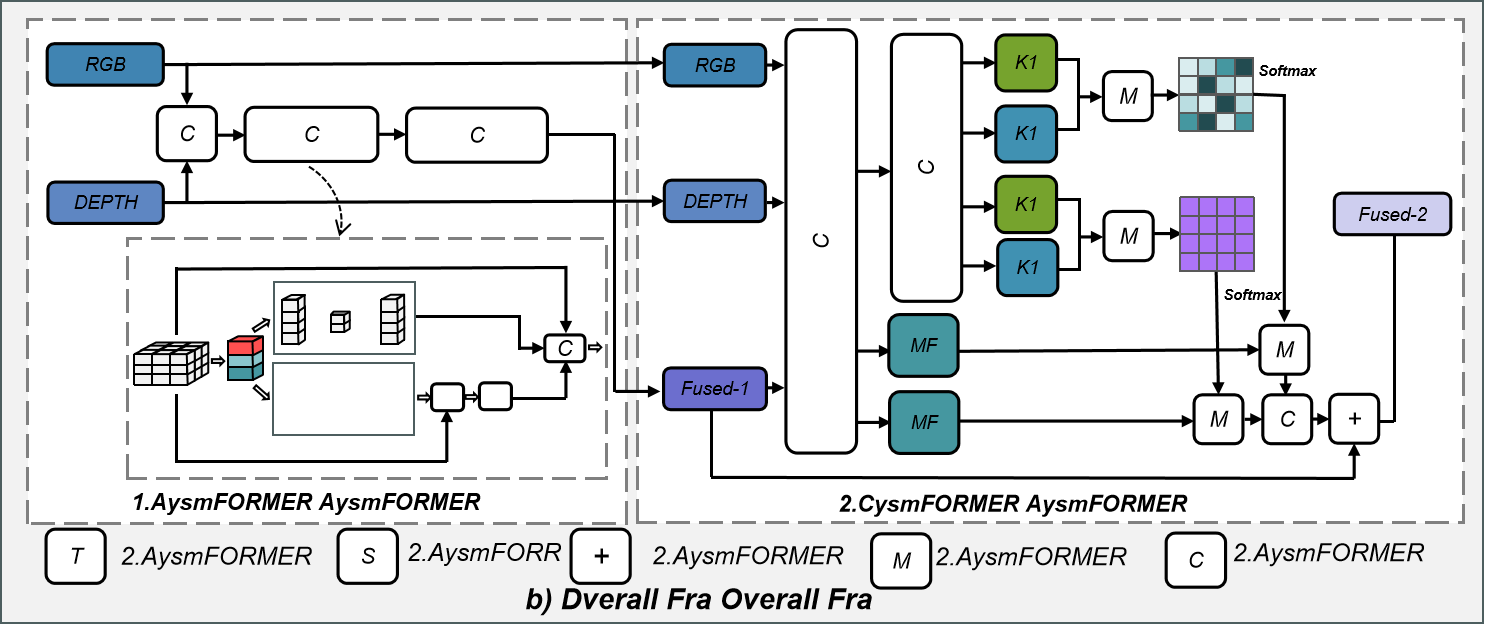
\includegraphics[width=\textwidth]{figures/跨模态融合结构.png}
	\caption{跨模态融合结构}
	\label{图:跨模态融合结构}
\end{figure}


\subsection{轻量级MLP解码器}
对于语义分割来说最重要的问题就是如何增大有效感受野。
对于Transformer encoder来说,由于self-attention有效感受野变得非常大,因此decoder不需要更多操作来提高有效感受野,也因此可以设计更加简单的decoder。

本文设计一个轻量级MLP解码器。
该解码器仅由MLP层组成,避免了其他方法中通常使用的手工设计和计算量较大的组件。
提出的全MLP解码器包括四个主要步骤。
首先,来自MiT编码器的多级特征Fi通过一个MLP层进行通道维度统一。
然后,在第二步中,特征被上采样到1/4大小,并进行拼接。
其次,采用MLP层来融合拼接后的特征F。
最后,另一个MLP层将融合后的特征输入,预测分割掩码M,分辨率为H/4 × W/4 × Ncls,其中Ncls是类别的数量。

可以将解码器表示为:
\begin{equation}
	\begin{aligned}
		&{\hat{F}_i = \text{Linear}(C_i, C)(F_i)}, \forall i\\
		&{{\hat{F}}_i = \text{Upsample}(\frac{W}{4} \times \frac{W}{4})({\hat{F}}_i)}, \forall i\\
		&{{F} = \text{Linear}(4C, C)(\text{Concat}({\hat{F}}_i})), \forall i\\
		&{{M} = \text{Linear}(C, N_{cls})({F})},
	\end{aligned}
	\label{eqn:mlp}
\end{equation}

其中,${\rm M}$是XX,$\text{Linear}(C_{in}, C_{out})(\cdot)$是XX,ZZ是XX。

如图如\ref{图:decoder}所示。
\begin{figure}[h]
	\centering
	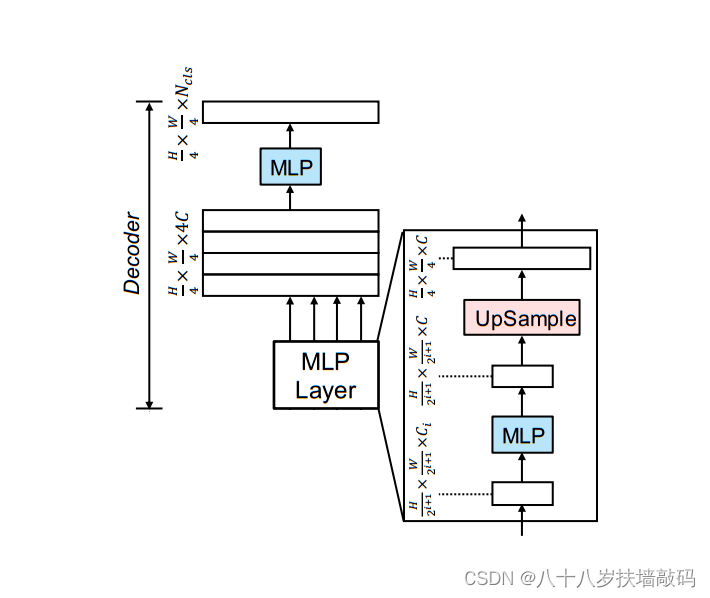
\includegraphics[width=\textwidth]{figures/decoder.png}
	\caption{decoder}
	\label{图:decoder}
\end{figure}







\section{实验结果分析}
\subsection{数据集与评价指标}
\textbf{(1)数据集}

本张使用公开数据集NYUv2和私有的地铁排爆数据集。
NYUv2是语义分割任务中使用最广泛的基准。
NYUv2原始数据集的数据来自3个城市的464个场景,并且绝大多数场景是室内场景,共894个类别标注。
通过对原始的语义标签扩展,有13类和40类两种版本用于语义分割。
根据做语义分割任务的大多数论文设定,本文采用40类的版本。
该版本的语义标签主要包括墙壁、地板、窗户、桌子和椅子等室内物体。
数据集主要包括彩色图片、深度图片以及标注图片。
1449张精细标注的图片被进一步分为795张和654张,分别用于训练和测试。图像尺寸640×480。
地铁排爆数据集是针对地铁排爆场景的自制数据集。
基础场景是某城市的某个地铁站点,通过在地铁月台和地铁车厢内部布置管状模拟爆炸物、模拟爆炸物疑似藏匿箱体等物体,模拟真实的地铁排爆场景。
该数据集一共有XX个语义分割类别,主要包括地铁闸机、地铁月台、地铁车厢内部座椅、模拟爆炸物、模拟爆炸物疑似藏匿箱体等物体。
数据集格式依照NYUv2数据集设置,主要包括彩色图片、深度图片以及标注图片。
XX张精细标注的图片被进一步分为XX张和XX张,分别用于训练和测试。图像尺寸640×480。
两个数据集的具体对比如XX所示。

\textbf{(2)评价指标}

实验中使用的X个指标来衡量语义分割算法的性能。
第一个是参数量(),该指标反应,该指标越低越好。
第二个是FLOPs。该指标越低越好。
第三个是Miou。该指标越高越好。

\subsection{参数设置}
本章算法使用pytorch框架,使用一台服务器进行训练和测试。该服务器装配有XX型号的CPU,四张RTX4090GPU,XX版本的CUDA。
表XX显示的是本章算法在NYUv2数据集和地铁排爆数据集上的详细参数设置。
在NYUv2数据集上,GPU数量设置为XX,批大小设置为XX,训练XX个epoch。
学习策略设置为XX,初始学习率设置为XX,学习率衰减参数设置为XX,
优化方法设置为XX,损失函数设置为XX。
在地铁排爆数据集上,GPU数量设置为XX,批大小设置为XX,训练XX个epoch。
学习策略设置为XX,初始学习率设置为XX,学习率衰减参数设置为XX,
优化方法设置为XX,损失函数设置为XX。
此外,在两个数据集的训练初始阶段,都采用数据增加对原始的彩色图片和深度图片进行处理,采用XX方法来提高模型的学习能力和泛化能力,但是在测试时,使用原始的图片,不涉及任何的数据增强,也不涉及任何对图片大小进行改变的操作。


\subsection{消融实验}
本小节通过在XX数据集上进行消融实验,验证XX算法中不同模块的有效性。
因此,本章的算法
XX模块表示XX。
XX模块表示XX。
XX模块表示XX。
%这里插入小消融实验的表格。
表XX展示了XX算法消融实验的结果。

\subsection{模型性能对比}




\subsection{对比实验}


\section{本章小结}
本章通过提出XX算法,该算法通过XX解决了XX问题。
实验结果表明,XX算法的XX指标相较基准算法分别降低了XX。


